% !TeX document-id = {5530719d-34df-4dd8-b4b5-e6ed092c2b36}
% !TeX program = pdflatex
% !BIB program = biber
\documentclass[sigconf,natbib=false]{acmart}

% Imports Ahoy

%\usepackage[dvipsnames]{xcolor}
%\usepackage{graphicx}
\usepackage{tikz}
\usepackage{varwidth}
\usetikzlibrary{arrows.meta, calc, fit, positioning}

\usepackage{etoolbox}
\usepackage[binary-units, per-mode=symbol]{siunitx}
\robustify\bfseries
\robustify\emph
%\robustify\uline
\sisetup{detect-all, range-phrase=--, range-units=single, detect-weight=true,detect-inline-weight=math, table-format=1.3}

\makeatletter
\let\MYcaption\@makecaption
\makeatother

\usepackage[font=footnotesize]{subcaption}

\makeatletter
\let\@makecaption\MYcaption
\makeatother

%\usepackage[basic]{complexity}
\usepackage[super,negative]{nth}

\usepackage[british]{babel}
\usepackage{csquotes}

\usepackage{booktabs}
%\usepackage[
%activate={true,nocompatibility},
%final,
%tracking=true,
%kerning=true,spacing=true
%]{microtype}
%\microtypecontext{spacing=nonfrench}

\usepackage[maxnames=2,maxbibnames=99,mincrossrefs=99,sortcites,style=numeric-comp
%,backend=biber
]{biblatex}
\addbibresource{papers-off.bib}
\addbibresource{confs-off.bib}
\addbibresource{books-off.bib}
\addbibresource{rfc.bib}
\addbibresource{misc.bib}

%\DeclareFieldFormat[inproceedings]{doi}{}
%\DeclareFieldFormat[article]{doi}{}
%\DeclareFieldFormat*{url}{}
%\DeclareFieldFormat[online]{url}{\mkbibacro{URL}\addcolon\space\url{#1}}
%\DeclareFieldFormat[report]{url}{\mkbibacro{URL}\addcolon\space\url{#1}}

%picky abt et al.
\usepackage{xpatch}

\usepackage{url}
\usepackage{hyperref}
\usepackage[nameinlink]{cleveref}
\newcommand{\crefrangeconjunction}{--}
\crefname{table}{table}{tables}

\DefineBibliographyStrings{english}{%
	andothers = {\emph{et al}\adddot}
}
\DeclareFieldFormat[inproceedings]{url}{}
\DeclareFieldFormat[article]{url}{}
%\DeclareFieldFormat[inproceedings]{doi}{}
%\DeclareFieldFormat[article]{doi}{}
%\DeclareFieldFormat[inproceedings]{editor}{}
%\DeclareFieldFormat[proceedings]{editor}{}
%\DeclareFieldFormat[article]{editor}{}

\newcommand{\fakepara}[1]{\noindent\textbf{#1:}}

% Official colours!

\definecolor{uofguniversityblue}{rgb}{0, 0.219608, 0.396078}

\definecolor{uofgheather}{rgb}{0.356863, 0.32549, 0.490196}
\definecolor{uofgaquamarine}{rgb}{0.603922, 0.72549, 0.678431}
\definecolor{uofgslate}{rgb}{0.309804, 0.34902, 0.380392}
\definecolor{uofgrose}{rgb}{0.823529, 0.470588, 0.709804}
\definecolor{uofgmocha}{rgb}{0.709804, 0.564706, 0.47451}

\definecolor{uofglawn}{rgb}{0.517647, 0.741176, 0}
\definecolor{uofgcobalt}{rgb}{0, 0.615686, 0.92549}
\definecolor{uofgturquoise}{rgb}{0, 0.709804, 0.819608}
\definecolor{uofgsunshine}{rgb}{1.0, 0.862745, 0.211765}
\definecolor{uofgpumpkin}{rgb}{1.0, 0.72549, 0.282353}
\definecolor{uofgthistle}{rgb}{0.584314, 0.070588, 0.447059}
\definecolor{uofgpillarbox}{rgb}{0.701961, 0.047059, 0}
\definecolor{uofglavendar}{rgb}{0.356863, 0.301961, 0.580392}

\definecolor{uofgsandstone}{rgb}{0.321569, 0.278431, 0.231373}
\definecolor{uofgforest}{rgb}{0, 0.317647, 0.2}
\definecolor{uofgburgundy}{rgb}{0.490196, 0.133333, 0.223529}
\definecolor{uofgrust}{rgb}{0.603922, 0.227451, 0.023529}

% End Imports

%\usepackage[english]{babel}
\usepackage{blindtext}

% Copyright
\renewcommand\footnotetextcopyrightpermission[1]{} % removes footnote with conference info
\setcopyright{none}
%\setcopyright{acmcopyright}
%\setcopyright{acmlicensed}
%\setcopyright{rightsretained}
%\setcopyright{usgov}
%\setcopyright{usgovmixed}
%\setcopyright{cagov}
%\setcopyright{cagovmixed}

\settopmatter{printacmref=false, printccs=false, printfolios=true}

% DOI
\acmDOI{12345}

% ISBN
\acmISBN{67890}

%Conference
\acmConference[SOSR '21]{}
%\acmYear{2021}
%\copyrightyear{}

%% {} with no args suppresses printing of the price
\acmPrice{}


\begin{document}
	\title{Revisiting the Classics: Online RL in the Programmable Data-Plane}
	
	%\titlenote{Produces the permission block, and copyright information}
	%\subtitle{Extended Abstract}
	
%	\author{Paper \# XXX, XXX pages}
	 \author{Kyle A. Simpson}
	 \orcid{0000-0001-8068-9909}
	 \affiliation{%
	   \institution{University of Glasgow}
	   \city{Glasgow} 
	   \country{Scotland}
	 }
	 \email{k.simpson.1@research.gla.ac.uk}
	 \author{Dimitrios P. Pezaros}
\orcid{0000-0003-0939-378X}
	 \affiliation{%
	\institution{University of Glasgow}
	\city{Glasgow} 
	\country{Scotland}
}
\email{Dimitrios.Pezaros@gla.ac.uk}
	
	% The default list of authors is too long for headers}
	\renewcommand{\shortauthors}{Simpson \emph{et al}.}
	
\begin{abstract}
Note: below text is just the UK systems workshop abstract I submitted.	
\end{abstract}
	
\maketitle
	
\section{Introduction}

Automatic optimisation, control, and defence of networks are at last becoming commonplace. Data-driven networking has led the charge in traffic optimisation, congestion control and packet classification via adaptive techniques such as Reinforcement Learning (RL), where every change and its measured effects further improve future decisions. Considering that the network evolves in its use and deployed protocols, this flexibility is essential. Yet data-driven methods suffer from a key weakness: they are dependent on both the recency and accuracy of input state. An out-of-date view of the world will lead to suboptimal choices, as will long processing times. These can result in worse performance and slower adaptation to the evolving network.

Programmable data-planes and in-switch compute, then, hold promise for integrating these new techniques in a feasible and efficient manner (beyond dedicated servers or virtualised network functions). For RL, key tasks include policy evaluation, online training, state collection, and action execution -- each of these introduces some degree of sensitivity to state accuracy. Ideally then, all logic would run on these programmable devices. Yet, there is often a finite budget in microcode/FPGA space, per-packet processing times, and available cores for execution. Moreover, necessary hardware, such as floating-point units, is unavailable in almost all cases.

The precise costs and trade-offs which operators and designers must make have yet to be identified. This follows from a design space explosion induced by many necessary workarounds. For instance, quantisation or fixed-point arithmetic will allow training and control on all devices, but introduces further questions: what degree of quantisation is most appropriate? What effect would this have on training accuracy, communications cost, or storage requirements? More concerns arise when we consider core allocation, local vs. distributed training, and reliable lightweight communication in multi-agent scenarios. In all cases, network operators will not consider tools which affect underlying traffic.

I aim to examine the effects of these choices on an existing RL-based DDoS attack mitigation system. To protect legitimate traffic, this controls packet drop and filtering for each flow using individual metrics observed by RL agents at ingress routers, and load measurements from several points along the path taken by the flow in question. The examined metrics include the throughput and latency of its individual components alongside system metrics: flow arrival-to-judgement time, and knowledge propagation time. Beyond this, it's crucial to identify what we can implement on pure P4-capable hardware. While extensions to P4 are fairly common in commodity hardware, the need for full design access (as in NetFPGA) or Micro-C (as in Netronome SmartNICs) represent a break from the clean, loop-free semantics of P4. As the market matures, these may represent different feature classes and price points.

I will discuss early development efforts (including challenges and results) on the Netronome Agilio SmartNIC, which supports the P4 language as well as some degree of arbitrary microcode. I intend to present how reinforcement learning execution and network telemetry will differ in the above metrics when compared to a vNF-based deployment (i.e., software on external commodity servers).

This paper contributes:
\begin{itemize}
	\item A thing (?? REFERENCE SECTION). Here's how that thing is utterly fantastic and will change the world, or not.
\end{itemize}

\section{Motivation}\label{sec:motivation}
\fakepara{Reinforcement learning in asynchronous environments}
RL techniques allow an \emph{agent} to learn how to iteratively interact with a system in an optimal fashion.
However, there is some degree of divergence between their theory and implementation.
Consider \cref{fig:state-slip}: the traditional formulation of a Markov decision process assumes that an agent receives a new view of the world's state at fixed time intervals, and then decides upon and executes an action instantly.
The reality is that state information takes time to traverse the network, service times are offset by how quickly hosts respond to interrupts and deserialise requests, and action preference lists are often computed via expensive policy approximations.
Action installation also incurs costs in fields such as network administration, initially to contact the controller and then for those actions to be installed via the control plane.

These delays (and variance thereof) add noise to the state-action mapping being learned, which has a potent reduction to learning rate and final accuracy, even for simple grid world tasks according to \textcite{DBLP:journals/firai/TravnikMSP18}.
They in turn show that reordering algorithmic steps can reduce these costs for online 1-step algorithms, but that reducing this further requires detailed agent-environment co-design.
This principle has influenced the design of real network use cases, such RL-based congestion-control algorithms~\parencite{DBLP:journals/corr/abs-1910-04054}, showing that asynchrony is necessary for high-speed applications.
Achieving this often requires that state measurements are combined or coalesced~\parencite{DBLP:journals/corr/abs-1910-04054,DBLP:journals/tnsm/SimpsonRP20} while expensive computations are ongoing.
`Stopping the world' in the algorithmic sense causes significant performance degradation, as inference takes up to \SI{30}{\milli\second} in the above work on congestion control, or any time-sensitive control problems.

\begin{figure}
	\begin{subfigure}{0.45\linewidth}
		\resizebox{\linewidth}{!}{
			\centering
			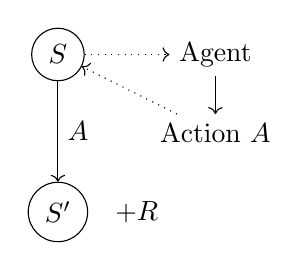
\begin{tikzpicture}
				\node[circle, draw] (state) {$S$};
				\node[circle, draw] (state') at ($(state) + (0, -2)$) {$S'$};
				
				\node (agent) at ($(2, 0) + (state)$) {Agent};
				\node[below of=agent] (action) {Action $A$};
				
				\node[right of=state'] {$+ R$};
				
				\draw[->] (state) -- (state') node[midway, right] {$A$};
				
				\draw[dotted, ->, bend left = 30] (state) -- (agent);
				\draw[->] (agent) -- (action);
				\draw[dotted, ->] (action) -- (state);
		\end{tikzpicture}}
		\caption{Theory: state measurement, action computation, and learning are zero-cost.}
	\end{subfigure}
	\begin{subfigure}{0.45\linewidth}
		\resizebox{0.75\linewidth}{!}{
			\centering
			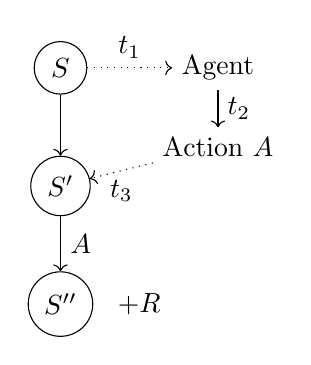
\begin{tikzpicture}
				\node[circle, draw] (state) {$S$};
				\node[circle, draw] (state') at ($(state) + (0, -1.5)$) {$S'$};
				\node[circle, draw] (state'') at ($(state') + (0, -1.5)$) {$S''$};
				
				\node (agent) at ($(2, 0) + (state)$) {Agent};
				\node[below of=agent] (action) {Action $A$};
				
				\node[right of=state''] {$+ R$};
				
				\draw[->] (state) -- (state') node[midway, right] {$\varnothing$};
				\draw[->] (state') -- (state'') node[midway, right] {$A$};
				
				\draw[dotted, ->, bend left = 30] (state) -- (agent) node[midway, above] {$t_1$};
				\draw[->] (agent) -- (action) node[midway, right] {$t_2$};
				\draw[dotted, ->] (action) -- (state') node[midway, below] {$t_3$};
		\end{tikzpicture}}
		\caption{Reality: costs of measurement and action lead to \emph{state drift}---over a time delay $t_1+t_2+t_3$, inaction transforms state $S$ into $S'$.}
	\end{subfigure}
	\caption{Asynchronous RL delays and state slippage (policy updates omitted).\label{fig:state-slip}}
\end{figure}

?? Find some cites citing the relevance of this problem wrt. self-driving cars, robotics, etc.

The solution we propose is to make use of the recent wave of programmable network devices to \emph{bring reinforcement learning to the data plane}---placing state measurement ($t_1$), low-cost decision-making processes ($t_2$), and controlled systems ($t_3$) as close to one another as possible.
In networks, actions are most likely to be installed on backbone switches, bump-in-the-wire NICs or middleboxes, and in the NICs of end-hosts.
Ideally, these functions which comprise an RL agent would all be collocated on the same chip or device, but this is easier said than done. 
Both programmable devices and the network environment make this more difficult, as we'll examine in the sequel.

\fakepara{Programmable hardware capabilities}
The introduction of the P4~\parencite{DBLP:journals/ccr/BosshartDGIMRSTVVW14} language has led to explosive growth in the research community surrounding in-network computation and offloading.
Providing a single language which is compatible with network devices of many form factors has been instrumental in the development of novel fine-grained traffic measurement approaches~\parencite{DBLP:conf/sigcomm/GuptaHCFRW18,DBLP:conf/sigcomm/ChenFKRR18,DBLP:conf/sosr/GhasemiBR17}.
However, this requires that there be a reasonably consistent interface and behaviour between device classes.
This need for underpins the \emph{Programmable Switch Architecture} (PSA)~\parencite{p4-psa}, which defines a conceptual model of match-action tables divided into ingress and egress pipelines.
The PSA presents a sensible lower bound on the device capabilities required to implement a P4 dataplane, but the reality is more complex and interesting.

We would be remiss to believe that the P4 and the PSA define all capabilities that programmable hardware can support.
Many compatible devices have legacies predating these developments, for instance many-core SOC-based Netronome SmartNIC~\parencite{netronome-smartnic}, and NetFPGA SUME~\parencite{DBLP:journals/micro/ZilbermanACM14} NICs.
The first of these compiles from P4$\rightarrow$Micro-C$\rightarrow$bytecode (with Micro-C externs), while the latter can combine the P4$\rightarrow$NetFPGA toolchain~\parencite{DBLP:conf/fpga/IbanezBMZ19} with arbitrary circuit externs---both exposing further device capabilities beyond the specification.
Even Intel Tofino~\parencite{barefoot-intel} ASICs, which architecturally mirror the PSA, expose additional matching capabilities and ALU functions via the Tofino Native Architecture.
Regardless, floating-point operations key to ML/RL workloads are very rarely supported outside of DL accelerators (which, in turn, lack packet switching functionality).
Moreover, the limited memory/block RAM and per-packet timing constraints endemic to these devices make this class of in-NIC offloading challenging.

Luckily, the task of bringing machine learning models to resource-constrained environments is well-studied.
Quantisation and alternative data formats have been suggested to make ML inference feasible on resource- and power-limited platforms, work around hardware constraints, or compute faster and more efficiently.
Lower bit-depths reduce memory footprints, and improve throughput in designs such as \emph{bfloat16}~\parencite{bfloat16-blog} in Google TPUs~\parencite{DBLP:journals/sigops/XieDMKVZT18}, \emph{hfp8}~\parencite{DBLP:conf/nips/SunCCWVSCZG19}, and other floating point formats~\parencite{DBLP:journals/corr/abs-2007-01530}.
In many cases, accuracy losses for doing so are negligible.
Much of this work goes further still towards integer~\parencite{tensorrt-8bit} or binarised~\parencite{DBLP:journals/corr/MiyashitaLM16,DBLP:conf/eccv/RastegariORF16,DBLP:journals/corr/KimS16,DBLP:conf/nips/HubaraCSEB16} representations, sacrificing dynamic range for simpler arithmetic operations.
This has the important side effect of making ML policy inference tractable on hardware without floating-point capabilities, which other works have leveraged to bring neural networks to the dataplane~\parencite{DBLP:journals/corr/abs-2009-02353,DBLP:conf/sigcomm/SanvitoSB18,DBLP:journals/corr/abs-1801-05731}.

To make RL workloads feasible under such constraints, we propose the use of quantised, fixed-point representations such as $Qm.n$, which allow us to evaluate and update policies using only integer arithmetic.
This is not only essential in performing this work, but also serves as a mechanism for reducing the processing and memory costs of function approximation ($t_2$, \cref{fig:state-slip}).
Crucially, we train our focus on devices with a low port density, such as SmartNICs and NetFPGA devices.
The designs of these devices make it reasonable to move policy processing \emph{outside of the packet pipeline}; SmartNICs expose many additional programmable cores, and NetFPGAs allow for the synthesis of independent functional units.
The main benefit of doing so is that core control logic can be moved as close to the device as possible \emph{without impacting packet processing rates}.
When combined with the above P4-driven techniques for in-network flow/device measurement, we at last have the mechanisms to collocate the key processes of an RL agent.
Moreover, the base P4 dataplane can be used to simplify parsing logic and offer runtime control over which flows/packets are monitored, alongside other packet actions.
This again fits our goals of integrating RL techniques directly within bump-in-the-wire installations and at end-hosts.

?? relate update/execute operations here? i.e., policy execute needs only ALU add, train needs add+mul+shr. or in RL section? Should that come first?

\fakepara{Online training}
Some problems either evolve over time in unpredictable ways, or cannot be easily modelled.
This can then make \emph{online} learning of the task an attractive prospect, using a single available stream of experience.
DNNs, particularly when used as the basis for an RL agent's policy, require vast amounts of experience to converge on an accurate parameter set.
In many problem domains, this equates to training from compute-years worth of distributed offline simulations, which is at odds with the need to adapt to changes in the underlying problem \emph{as they happen}.
Achieving stable learning requires sizeable batches of gradients to be computed, potentially using the entire experience replay from each simulation.
Still, the computational cost of gradient computation via backpropagation is significant on embedded hardware.

To then achieve \emph{online} learning, we return our focus to older \emph{classical} reinforcement learning methods.
In particular, we suggest tile-coding~\cite[pp. \numrange{217}{221}]{RL2E}, with one-step temporal-difference learning algorithms such as Sarsa or Q-learning~\cite[pp. \numrange{129}{132}]{RL2E}.
These choices have important benefits for in-NIC execution.
Simpler function approximators do not require batches of inputs to learn in a more stable way, negating the additional memory required to store experience replays.
Tile-coding in particular admits many optimisations, being an embarrassingly parallel problem.
Furthermore, gradient calculation is trivial for linear methods like tile coding, particularly when compared to the computational cost of backpropagation required by neural networks.
Finally, the choice of single-step algorithms (as opposed to $n$-step or Monte Carlo methods) bounds the amount of per-trace state required for online learning to just the last state-action pair.

?? Probably want some cites on the need for batching in NN methods, even though this is understood. DL book?

\fakepara{To-be-organised}
Interesting thing I realised from \textcite{DBLP:conf/sigcomm/NeugebauerAZAL018}: GPU and NIC might cause IOMMU contention? Making line-rate offload of DDN to GPU impractical. Unsure if I want to twin this with later measurements/plots.

\section{Background}

\subsection{Classical Reinforcement Learning}
?? Move into background parent section?

?? RL~\parencite{RL2E}

?? Use this to explain differences between the modern state of the art and older works.

?? Probably give a rough introduction to the algorithm, show how computation needs only addition---particularly when using Qm.n fixed point.

\subsection{Hmm..}
Should motivation be in here? Unsure what other preliminaries need to be explained.

\section{Design and Implementation}\label{sec:design}
Based on the design principles, problems, and potential solutions outlined throughout \cref{sec:motivation}, we present our design for an in-NIC, task-independent, online reinforcement learning system.
\Cref{fig:netro-arch} outlines our design and implementation on Netronome SmartNIC hardware in pursuit of this goal.
At a high level, ...

\subsection{Policy Storage}
?? Blocks of dense quantised tiles: each an action preference list.

?? Tiling data is split into regions of memory based on access time: higher-dimension tilings are sent to further NUMA regions (EMEM/IMEM).

\subsection{Action Computation}
?? Split across MEs.

?? each ME can then subdivide by factor of 4 among contexts.

\subsection{Communication}
?? Free-list of packet handles shared between P4 pipeline threads for state/config/action handover.

?? multi-producer-multi-consumer -- rings used to signal cores, place work, etc., combined with above free-list

?? used for both directions of communication.

\subsection{Notes from PGR}

The main gist of this design is that RL operations \emph{do not happen on the core data path}, which ensures that action computation, installation, and updates don't stall packet transmission or affect throughput.
In the default deployment of a P4 packet processing pipeline, several of these cores go unused, making this paradigm possible.
These dedicated cores (\emph{micro-engines} grouped by \emph{island} in NFP terminology) are then responsible for processing requests, computing actions, and updating the underlying policy in real time.
The main interaction model is that platform-specific IPC mechanisms (message rings) are used to \emph{push} configuration, state vectors, and reward measurements to the RL system.
These same mechanisms are used by other cores on the same device to \emph{pull} output actions from the RL system.
Both input and output can occur on any other core of the device, i.e., as part of P4 \texttt{extern} plugins, while the P4 control plane itself provides granular control over which flows are monitored or affected.
An input state vector \emph{always} induces an action, and if desired updates the policy using either an included reward or one retrieved from memory according to a (configurable) key in the state.
Runtime reconfiguration and interaction occur via the control and/or dataplane: the ease of use of the P4 pipeline's match and custom protocol parsers, combined with the dedicated input pipe to the NIC's controller (the host machine), allow these to be cleanly separated or combined as needed.

?? Expand: this is based on PGR Year 3 atm.

\subsection{Targetting other device classes}
While this design caters primarily to Netronome's SmartNIC devices, many aspects of this design have clear analogues in NICs of similar form-factor, such as their close NetFPGA SUME cousins.
For instance, the availability of other cores can be handled by designing additional off-path functional units, much like the floating-point adders used by \textcite{DBLP:conf/isca/LiLYCSH19}.
Rather than general-purpose cross-core communication, an RL functional unit would be hard-wired to and from the custom actions that interface with it, using the P4$\rightarrow$NetFPGA toolchain to offer the base framework and granular control over packet and flow selection.

?? Fill out above with more specific instances.

Bringing this to high-port density devices such as Intel Tofino-powered switches is more difficult.
As discussed in \cref{sec:motivation}, Tofino ASICs map closely to the P4 PSA, meaning that there are no spare asynchronous general-purpose compute units to place this work on.
A potential solution is to divide RL actions across several received packets (i.e., iteratively computing a portion of the action preference list each time) until any further work would delay outbound transmission.
This, however, would introduce new issues surrounding concurrent accesses, work splitting, and altered timescales for learning: we leave their treatment and examination to future work.

\section{Techniques}

What does the hardware give us, and what can we assume are present on many other classes of device?
\begin{itemize}
	\item 96-core (\emph{management engine}, ME) (? check), grouped into \emph{islands} based on local capabilities. Fast transfer between MEs on same island (\emph{nearest neighbour registers}, NNRs)
	
	\begin{itemize}
		\item Multicore model common.
		\item Arch-specific: one program per ME. Enables cooperative scheduling between \numrange{4}{8} threads, zero-cost context switch due to register file (below).
	\end{itemize}

	\item Explicit memory hierarchy:
	
	\begin{itemize}
		\item Large register file split disjointly between threads. (likely common)
		\item Transparent cache.
		\item In order of speed? Reg file, External Mem
	\end{itemize}

	\item One program to a core---enables cooperative scheduling with zero-cost context switches.
	
\end{itemize}
Now how do we make this work?
\begin{itemize}
	\item No floating point math. Solution? Quantisation (cite some other papers who've used this to decent effect).
	
	\item Bump-in-the-wire design for SmartNIC.
	
	\item P4 for easy packet parsing, control packet extraction, passthrough and manipulation of other traffic.
	
	\item RL Island keeps freelist, P4 PIF Islands copy packets over (could in theory hack P4 firmware micro-C libraries to stop freeing resources and just pass those?).
	
	\item Control packets marked by custom \emph{experimenter} DSCP (as in \textcite{DBLP:conf/isca/LiLYCSH19}). Infrastructure can ensure that only trusted internal nodes can produce such packets.
	
	\item Control allows adaptation to any policy design assuming standard tile-coding, for any target application. Policies may be installed via block copy, or trained online. (So long as policy meets compiled maximum dimensions, constraints.)
	
	\item (not impl'd yet) How does state work? Packet passed in over work queue to control ME. source can be either the network (same mechanism as control packets)
	
	\item (not impl'd yet) How do actions work? 2 options.
	\begin{enumerate}
		\item Produce packet on wire according to config (custom format).
		\item Pass packet to local island/ME (requires both config and custom build).
	\end{enumerate}

	\item Built with \Textcite{DBLP:journals/tnsm/SimpsonRP20} in mind, but applicable to any RL application.
	
	\item New PDPs have encryption primitives: scope to include authentication etc. around control packets.
	
	\item (Not impl'd yet) Event loop can easily run on Control ME: timing APIs exposed to generate periodic events in lieu of something like \textcite{DBLP:conf/hotnets/IbanezABM19}.
\end{itemize}

\begin{figure}
	\centering
	\resizebox{\linewidth}{!}{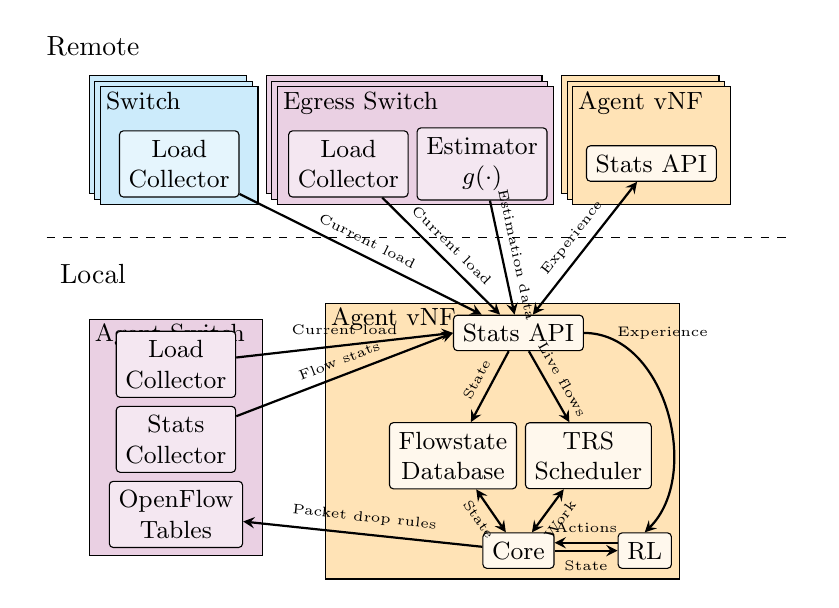
\begin{tikzpicture}
		\node(remote){Remote};
		
		%%%
		
		\node[below=0.05 of remote](swpos){};
		\node[fill=white!80!uofgcobalt, draw=black, minimum height=1.5cm, minimum width=2cm, below right= 0.1 of swpos.north west](sw1){};
		\node[fill=white!80!uofgcobalt, draw=black, minimum height=1.5cm, minimum width=2cm, below right= 0.1 of sw1.north west](sw2){};
		\node[fill=white!80!uofgcobalt, draw=black, minimum height=1.5cm, minimum width=2cm, below right= 0.1 of sw2.north west](switch){};
		\node[below right, inner sep=2pt] at (switch.north west) {\small Switch};
		\node[fill=white!90!uofgcobalt, draw, rectangle, rounded corners=0.05cm, above=0.1] (oswlc) at (switch.south) {\begin{varwidth}{1.5 cm}\small \centering Load\\Collector\end{varwidth}};
		
		%
		
		\node[right=2 of swpos](epos){};
		\node[fill=white!80!uofgthistle, draw=black, minimum height=1.5cm, minimum width=3.5cm, below right= 0.1 of epos.north west](e1){};
		\node[fill=white!80!uofgthistle, draw=black, minimum height=1.5cm, minimum width=3.5cm, below right= 0.1 of e1.north west](e2){};
		\node[fill=white!80!uofgthistle, draw=black, minimum height=1.5cm, minimum width=3.5cm, below right= 0.1 of e2.north west](egress){};
		\node[below right, inner sep=2pt] at (egress.north west) {\small Egress Switch};
		\node[fill=white!90!uofgthistle, draw, rectangle, rounded corners=0.05cm, above=0.1] (eglc) at ($(egress.south) + (-0.85,0)$) {\begin{varwidth}{1.5 cm}\small \centering Load\\Collector\end{varwidth}};
		\node[fill=white!90!uofgthistle, draw, rectangle, rounded corners=0.05cm, right=0.1] (egest) at (eglc.east) {\begin{varwidth}{1.5 cm}\small \centering Estimator\\$g(\cdot)$\end{varwidth}};
		
		%
		
		\node[right=3.5 of epos](apos){};
		\node[fill=white!60!uofgpumpkin, draw=black, minimum height=1.5cm, minimum width=2cm, below right= 0.1 of apos.north west](a1){};
		\node[fill=white!60!uofgpumpkin, draw=black, minimum height=1.5cm, minimum width=2cm, below right= 0.1 of a1.north west](a2){};
		\node[fill=white!60!uofgpumpkin, draw=black, minimum height=1.5cm, minimum width=2cm, below right= 0.1 of a2.north west](otheragent){};
		\node[below right, inner sep=2pt] at (otheragent.north west) {\small Agent vNF};
		\node[fill=white!90!uofgpumpkin, draw, rectangle, rounded corners=0.05cm, above=0.3] (oasa) at (otheragent.south) {\begin{varwidth}{1.5 cm}\small \centering Stats API\end{varwidth}};
		
		%
		
		\node[below=2.3 of remote.west](linestart){};
		\path let \p1 = (linestart) in node (lineend) at (9,\y1){};
		\draw [dashed] (linestart) -- (lineend);
		
		%%%
		
		\node[below=2.4 of remote](local){Local};
		
		%%%
		
		\node[below=0.25 of local](aswpos){};
		\node[fill=white!80!uofgthistle, draw=black, minimum height=3cm, minimum width=2.2cm, below right= 0.1 of aswpos.north west](aswitch){};
		\node[below right, inner sep=2pt] at (aswitch.north west) {\small Agent Switch};
		\node[fill=white!90!uofgthistle, draw, rectangle, rounded corners=0.05cm, above=0.1] (aswoft) at (aswitch.south) {\begin{varwidth}{1.5 cm}\small \centering OpenFlow\\Tables\end{varwidth}};
		\node[fill=white!90!uofgthistle, draw, rectangle, rounded corners=0.05cm, above=0.1] (aswsc) at (aswoft.north) {\begin{varwidth}{1.5 cm}\small \centering Stats\\Collector\end{varwidth}};
		\node[fill=white!90!uofgthistle, draw, rectangle, rounded corners=0.05cm, above=0.1] (aswlc) at (aswsc.north) {\begin{varwidth}{1.5 cm}\small \centering Load\\Collector\end{varwidth}};
		
		%
		
		\node (avfpos) at ($(aswpos) + (3,0.2)$){};
		\node[fill=white!60!uofgpumpkin, draw=black, minimum height=3.5cm, minimum width=4.5cm, below right= 0.1 of avfpos.north west](avf){};
		\node[below right, inner sep=2pt] at (avf.north west) {\small Agent vNF};
		\node[fill=white!90!uofgpumpkin, draw, rectangle, rounded corners=0.05cm, below=0.15] (avfsa) at ($(avf.north) + (0.2,0)$) {\begin{varwidth}{1.5 cm}\small \centering Stats API\end{varwidth}};
		\node[fill=white!90!uofgpumpkin, draw, rectangle, rounded corners=0.05cm, below=0.9] (avfdb) at (avfsa.south west) {\begin{varwidth}{1.5 cm}\small \centering Flowstate\\Database\end{varwidth}};
		\node[fill=white!90!uofgpumpkin, draw, rectangle, rounded corners=0.05cm, right=0.1] (avfsched) at (avfdb.east) {\begin{varwidth}{1.5 cm}\small \centering TRS\\Scheduler\end{varwidth}};
		\node[fill=white!90!uofgpumpkin, draw, rectangle, rounded corners=0.05cm, below=2.3] (avfcore) at (avfsa.south) {\begin{varwidth}{1.5 cm}\small \centering Core\end{varwidth}};
		\node[fill=white!90!uofgpumpkin, draw, rectangle, rounded corners=0.05cm, right=0.8] (avfrl) at (avfcore.east) {\begin{varwidth}{1.5 cm}\small \centering RL\end{varwidth}};
		
		%%%
		
		\tikzset{>=stealth}
		
		\draw[thick, ->] (aswlc) -- (avfsa.west) node[midway,above] {\tiny Current load};
		\draw[thick, ->] (aswsc) -- (avfsa.west) node[midway,sloped, above] {\tiny Flow stats};
		
		\draw[thick, ->] (oswlc) -- (avfsa) node[midway,above, sloped] {\tiny Current load};
		
		\draw[thick, ->] (eglc) -- (avfsa) node[midway,above, sloped] {\tiny Current load};
		\draw[thick, ->] (egest) -- (avfsa) node[midway,above, sloped] {\tiny Estimation data};
		
		\draw[thick, <->] (oasa) -- (avfsa) node[midway,above, sloped] {\tiny Experience};
		
		\draw[thick, ->] (avfsa) -- (avfdb) node[midway,above, sloped] {\tiny State};
		\draw[thick, ->] (avfsa) -- (avfsched) node[midway,above, sloped] {\tiny Live flows};
		
		\draw[thick, ->] (avfcore) -- (aswoft) node[midway,above, sloped] {\tiny Packet drop rules};
		\draw[thick, <->] (avfcore) -- (avfdb) node[midway,below, sloped] {\tiny State};
		\draw[thick, <->] (avfcore) -- (avfsched) node[midway,below, sloped] {\tiny Work};
		\draw[thick, <-] ($(avfcore.east) + (0,0.1)$) -- ($(avfrl.west) + (0,0.1)$) node[midway,above, sloped] {\tiny Actions};
		\draw[thick, ->] (avfcore) -- (avfrl) node[midway,below, sloped] {\tiny State};
		
		\draw[thick, ->] (avfsa.east) to [out=0, in=45] (avfrl.north);
		\node[right=0.3] at (avfsa.east) {\tiny Experience};
		\end{tikzpicture}}
	\caption{
		System architecture  for our RL-driven DDoS defence system.
		\label{fig:sys-arch}
	}
\end{figure}

\begin{figure}
	\centering
	\resizebox{1.2\linewidth}{!}{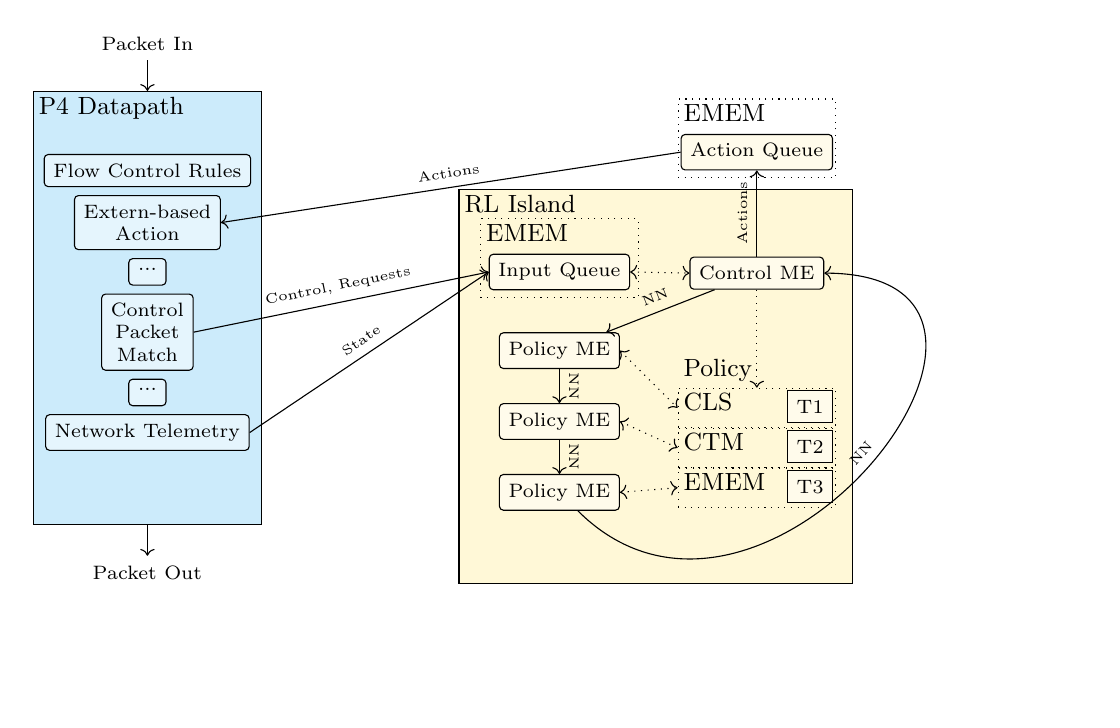
\begin{tikzpicture}
			\node (sw2) {};
			
			\node[fill=white!80!uofgcobalt, draw=black, minimum height=5.5cm, minimum width=2.9cm, below right= 0.1 of sw2.north west](p4-master){};
			\node[below right, inner sep=2pt] at (p4-master.north west) {\small P4 Datapath};
			\node[fill=white!90!uofgcobalt, draw, rectangle, rounded corners=0.05cm, below=0.8] (p4-rules) at (p4-master.north) {\begin{varwidth}{2.5 cm}\scriptsize \centering Flow Control Rules\end{varwidth}};
			\node[fill=white!90!uofgcobalt, draw, rectangle, rounded corners=0.05cm, below=0.1] (n1) at (p4-rules.south) {\begin{varwidth}{2.5 cm}\scriptsize \centering Extern-based Action\end{varwidth}};
			\node[fill=white!90!uofgcobalt, draw, rectangle, rounded corners=0.05cm, below=0.1] (n2) at (n1.south) {\begin{varwidth}{2.5 cm}\scriptsize \centering ...\end{varwidth}};
			\node[fill=white!90!uofgcobalt, draw, rectangle, rounded corners=0.05cm, below=0.1] (oswlc) at (n2.south) {\begin{varwidth}{1.5 cm}\scriptsize \centering Control Packet Match\end{varwidth}};
			\node[fill=white!90!uofgcobalt, draw, rectangle, rounded corners=0.05cm, below=0.1] (n3) at (oswlc.south) {\begin{varwidth}{2.5 cm}\scriptsize \centering ...\end{varwidth}};
			\node[fill=white!90!uofgcobalt, draw, rectangle, rounded corners=0.05cm, below=0.1] (n4) at (n3.south) {\begin{varwidth}{2.5 cm}\scriptsize \centering Network Telemetry\end{varwidth}};
			
			
			
			\node (pkt-text) at ($(p4-master.north) + (0.0,0.6)$) {\begin{varwidth}{2.5 cm}\scriptsize \centering Packet In\end{varwidth}};
			
			\node (pkt-text-out) at ($(p4-master.south) + (0.0,-0.6)$) {\begin{varwidth}{2.5 cm}\scriptsize \centering Packet Out\end{varwidth}};
			
			\node[fill=white!80!uofgsunshine, draw=black, minimum height=5cm, minimum width=5cm](rli) at ($(p4-master.east) + (5, -1)$){};
			\node[below right, inner sep=2pt] at (rli.north west) (rli-text) {\small RL Island};
			
			\node[draw=black, dotted, minimum height=1cm, minimum width=2cm](wq-out) at ($(rli-text.south) + (0.5,-0.5)$){};
			\node[below right, inner sep=2pt] at (wq-out.north west) {\small EMEM};
			\node[fill=white!90!uofgsunshine, draw, rectangle, rounded corners=0.05cm, above=0.1] (wq-in) at (wq-out.south) {\begin{varwidth}{2.5 cm}\scriptsize \centering Input Queue\end{varwidth}};
			
			\node[fill=white!90!uofgsunshine, draw, rectangle, rounded corners=0.05cm, above=0.1] (loop) at ($(wq-out.east) + (1.5,-0.5)$) {\begin{varwidth}{2.5 cm}\scriptsize \centering Control ME\end{varwidth}};
			
			\node[draw=black, dotted, minimum height=1cm, minimum width=2cm](wq-act) at ($(loop.north) + (0.0,1.5)$){};
			\node[below right, inner sep=2pt] at (wq-act.north west) {\small EMEM};
			\node[fill=white!90!uofgsunshine, draw, rectangle, rounded corners=0.05cm, above=0.1] (wq-actin) at (wq-act.south) {\begin{varwidth}{2.5 cm}\scriptsize \centering Action Queue\end{varwidth}};
			
			\node[draw=black, dotted, minimum height=0.5cm, minimum width=2cm](policy-cls-out) at ($(loop.south) + (0,-1.5)$){};
			\node[below right, inner sep=2pt] at (policy-cls-out.north west) {\small CLS};
			\node[above right, inner sep=2pt] at (policy-cls-out.north west) {\small Policy};
			\node[draw=black, dotted, minimum height=0.5cm, minimum width=2cm](policy-ctm-out) at ($(policy-cls-out.south) + (0,-0.25)$){};
			\node[below right, inner sep=2pt] at (policy-ctm-out.north west) {\small CTM};
			\node[draw=black, dotted, minimum height=0.5cm, minimum width=2cm](policy-emem-out) at ($(policy-ctm-out.south) + (0,-0.25)$){};
			\node[below right, inner sep=2pt] at (policy-emem-out.north west) {\small EMEM};
			
			\node[fill=white!90!uofgsunshine, draw, rectangle, above=0.1, below left= 0.05] (t1) at (policy-cls-out.north east) {\begin{varwidth}{2.5 cm}\scriptsize \centering T1\end{varwidth}};
			\node[fill=white!90!uofgsunshine, draw, rectangle, above=0.1, below left= 0.05] (t2) at (policy-ctm-out.north east) {\begin{varwidth}{2.5 cm}\scriptsize \centering T2\end{varwidth}};
			\node[fill=white!90!uofgsunshine, draw, rectangle, above=0.1, below left= 0.05] (t3) at (policy-emem-out.north east) {\begin{varwidth}{2.5 cm}\scriptsize \centering T3\end{varwidth}};
			
			\node[fill=white!90!uofgsunshine, draw, rectangle, rounded corners=0.05cm, above=0.1] (po-me-1) at ($(wq-out.south) + (0,-1.0)$) {\begin{varwidth}{2.5 cm}\scriptsize \centering Policy ME\end{varwidth}};
			
			\node[fill=white!90!uofgsunshine, draw, rectangle, rounded corners=0.05cm, above=0.1] (po-me-2) at ($(po-me-1.south) + (0,-1.0)$) {\begin{varwidth}{2.5 cm}\scriptsize \centering Policy ME\end{varwidth}};
			
			\node[fill=white!90!uofgsunshine, draw, rectangle, rounded corners=0.05cm, above=0.1] (po-me-3) at ($(po-me-2.south) + (0,-1.0)$) {\begin{varwidth}{2.5 cm}\scriptsize \centering Policy ME\end{varwidth}};
			
			\draw[->] (oswlc.east)  to node[midway, above, sloped] {\tiny Control, Requests} (wq-in.west);
			\draw[->] (n4.east)  to node[midway, above, sloped] {\tiny State} (wq-in.west);
			\draw[<->, dotted] (wq-in.east)  to (loop.west);
			\draw[->, dotted] (loop.south) to (policy-cls-out);
			
			\draw[->] (loop.north)  to node[midway, above, sloped] {\tiny Actions} (wq-actin.south);
			
			\draw[->] (wq-actin.west)  to node[midway, above, sloped] {\tiny Actions} (n1.east);
			
			\draw[<->, dotted] (po-me-1.east) to (policy-cls-out.west);
			\draw[<->, dotted] (po-me-2.east) to (policy-ctm-out.west);
			\draw[<->, dotted] (po-me-3.east) to (policy-emem-out.west);
			
			\draw[->] (pkt-text)  to  (p4-master.north);
			\draw[->] (p4-master.south)  to  (pkt-text-out);
			
			\draw[->] (loop) to node[midway, above, sloped] {\tiny NN} (po-me-1);
			\draw[->] (po-me-1) to node[midway, above, sloped] {\tiny NN} (po-me-2);
			\draw[->] (po-me-2) to node[midway, above, sloped] {\tiny NN} (po-me-3);
			\draw[->] (po-me-3) to [out=-45,in=0,looseness=2] node[midway, above, sloped] {\tiny NN} (loop);
	\end{tikzpicture}}
	\caption{Architecture for generalised RL agent on Netronome hardware.\label{fig:netro-arch}}
\end{figure}

\section{Evaluation}

How do we evaluate this without looking into classification performance?
\begin{itemize}
	\item Analytically?
	\begin{enumerate}
		\item Prove that tile splitting scheme over memory hierarchy can improve performance.
		\begin{itemize}
			\item Hit rate of different tiles according to tile dimensionality?
			\item Access time for each tier of memory hierarchy.
		\end{itemize}
	\end{enumerate}
	\item Experimentally?
	\begin{enumerate}
		\item Create ``VNF'' testbed: mirror traffic from switch to a host for telemetry processing/flow state. Send flow state over to another node who computes RL actions. RL actions installed on switch.
		\begin{itemize}
			\item Why not co-host RL computation with telemetry? Could be separate functions, could want to ensure that neither impacts the performance of the other.
		\end{itemize}
		\item Create ``PDP'' testbed: Load firmware, pass in traffic. Traffic processing/action compute/table mod occurs in PDP.
		\item What traffic? Healthy mix of attack (UDP), Discord legit Opus VoIP traffic, HTTP bulk-transfer traffic.
		\item Measure $t_{1 \cdots 3}$ according to \cref{fig:state-slip} in both VNF and PDP contexts.
		\begin{description}
			\item[$t_1$]
			\begin{description}
				\item[PDP] Packet ingress $\rightarrow$ INT Island $\rightarrow$ State arrival in Control ME.
				\item[VNF] Packet mirror time $\rightarrow$ telemetry VNF $\rightarrow$ state arrival in agent vnf.
			\end{description}
		
			\item[$t_2$]
			\begin{description}
				\item[PDP] Time to compute action over parallel Policy MEs (RL Island, SmartNIC).
				\item[VNF] Time to compute action in host program (on VNF) from received state.
			\end{description}
		
			\item[$t_3$]
			\begin{description}
				\item[PDP] Modify local tables across ME/Island boundaries (same device), verify rule present (or get ACK).
				\item[VNF] Generate OpenFlow control messages, send OF message to switch, verify rule present (or get ACK).
			\end{description}
		\end{description}
		\item HYPOTHESIS: PDP will present a reduction in these three times for per-flow state.
		\item QUESTION: Does same apply to learning?
		\item NOTE: since we're not actually assessing the \emph{quality} of output decisions, we can cut corners on what data is sent out and where. I.e., in-band network telemetry island can be skipped, if we move over representative volumes of state to/from the RL island with approximately correct delay as recorded by other studies.
	\end{enumerate}
\end{itemize}
I can think of one way to evaluate this if we employ classification performance:
\begin{enumerate}
	\item Run the existing work~\parencite{DBLP:journals/tnsm/SimpsonRP20}, acquire a policy for one node after full info sharing.
	\item Load this policy onto the RL Island (\cref{fig:netro-arch}).
	\item Either feed in raw state packets, or feed in traffic if we can get INT working.
	\item For each level of quantisation needed, examine average performance.
	\item Don't compare against old numbers for final perf: use a ``VNF'' setup similar to above---this will probably suffer a bit compared to old results, where everything was on the same machine. Make it relative/normalised.
\end{enumerate}

\section{Bullets on (intended) design.}
See also: \cref{fig:netro-arch}.
\begin{itemize}
	\item High-level overview.
	\begin{itemize}
		\item RL operations \emph{do not happen on the core path}.
		\item Another island (or set of cores) is dedicated to handling inputs, configuration, computation.
		\item Cross-island communication happens over \emph{rings} (Netronome-specific).
		\begin{itemize}
			\item E.g., this is how the P4 firmware propagates rules from master island to P4 workers.
			\item My impl.\ specific---shared freelist for memory pointers in EMEM.
		\end{itemize}
		\item Controller is \emph{always} co-hosted, interfaces over PCI-e. This also applies to Barefoot Tofino.
	\end{itemize}
	\item Policy configuration.
	\begin{itemize}
		\item (Re)-configurable at runtime.
		\item Custom DSCP marker acts as indicator of RL packets (i.e., bother with parsing past UDP).
		\item P4 parser extracts headers, parser state and payload passed over ring to another core dedicated to RL operations.
		\item Policy dimensions, size, action count, tiling strategies, learning parameters ($\alpha, \gamma, \epsilon$, related falloffs) can all be chosen and changed live.
	\end{itemize}
	\item State Handling.
	\begin{itemize}
		\item State input to model \emph{always} should produce an action.
		\item State vectors should come from elsewhere on the device: this may either be a dedicated island/core cluster (i.e., also performing INT management), or it may be a packet from the network.
	\end{itemize}
	\item Action Handling.
	\begin{itemize}
		\item A state vector is tile coded, action probabilities are produced, and an action is chosen according to current choice of $\epsilon$ (exploration parameter).
		\item \emph{Open question: how to configure action destination? This should either be another core (after an optional transformation), a packet sent out to a destination, maybe talk back to the controller.}
	\end{itemize}
	\item Learning.
	\begin{itemize}
		\item \emph{Open question: how to safely \& reasonably map state back to incoming rewards?}
		\item \emph{Open question: Can/should this also support on-chip reward signals?}
	\end{itemize}
\end{itemize}

\section{What's implemented 'til now?}
System?
\begin{itemize}
	\item Core-to-core communication.
	\item P4 parser for relevant packets.
	\item Packet copy + handoff from P4 to RL MEs.
	\item Dynamic base configuration.
	\item Dynamic tiling configuration.
	\item Policy installation via block-copy.
	\item Packet generation for above config functions, as well as policy quantisation and splitting.
	\item Tile-coding of quantised states on-chip, and state packet receipt.
	\item Action computation on-chip.
	\item Rudimentary, single-core training.
\end{itemize}

Experiments?
\begin{itemize}
	\item Policy quantisation divergence \& accuracy (via mininet).
	\item Measure DPDK SmartNIC RTT as a lower bound on controller access time.
	\begin{itemize}
		\item Same mechanism applies to other manufacturers (Barefoot), so generalisable.
		\item My results are non-DPDK, but there is a good study~\parencite{DBLP:conf/sigcomm/NeugebauerAZAL018} on exactly this.
	\end{itemize}
	\item Measure basic on-switch times: ring-ring communication, tile-coding cost, action compute cost, learning cost.
\end{itemize}

Known/understood (but not implemented)?
\begin{itemize}
	\item Figure out PIF rule installation.
	\begin{itemize}
		\item Not doable through P4 na\"{i}vely. Handing back rules to controller is expensive: need another action to deliberately use its own hash table etc., then batch back as faster P4 rules.
	\end{itemize}
\end{itemize}

\section{Intermediate steps?}
System?
\begin{itemize}
	\item Setup other core as event source.
	\begin{itemize}
		\item \emph{\num{2} week.}
		\item Idea: proxy for idea of INT core mentioned elsewhere, combined with the main periodic event sending that the last RL work relied upon. So, say "you can put that state management and extraction on another core, here's what the comms cost is" or similar.
	\end{itemize}
	\item Fixes to hash table use, signalling.
	\begin{itemize}
		\item \emph{\num{1} week.}
		\item Blocks progress on optimisation, correct multi-stream RL.
	\end{itemize}
	\item Optimise/parallelise action compute/learning.
	\begin{itemize}
		\item \emph{\num{2} week.}
		\item Value? Proves this approach can scale according to resource availability/demand on the deployment device, at compile-time anyhow.
	\end{itemize}
\end{itemize}

Experiments?
\begin{itemize}
	\item Measure sum of times $t_{1...3}$ described elsewhere.
	\begin{itemize}
		\item \emph{\num{1} week.}
		\item Currently have individual, need ``end-to-end''.
	\end{itemize}
	\item Throughput impact testing.
	\begin{itemize}
		\item \emph{\num{1} week.}
		\item Requires current impl, creation of basic testbed and packet forwarding setup.
		\item Use-case independent.
	\end{itemize}
	\item Measure execution, training costs for varying policy sizes.
	\begin{itemize}
		\item \emph{\num{1.5} weeks.}
		\item Policies need not be meaningful, and can be garbage data. Use-case independent.
		\item Partially blocked on multicore accelerated/optimised execution.
	\end{itemize}
	\item Measure rule installation cost on different platforms.
	\begin{itemize}
		\item \emph{\num{1.5} weeks.}
		\item Blocked on creation of basic testbed and packet forwarding setup.
	\end{itemize}
	\item Investigate stationarity.
	\begin{itemize}
		\item \emph{\numrange{2}{3} weeks.}
		\item Requires full use-case implementation.
		\item Requires careful thought about sensible changes to normality.
		\item Might be bolstered by comparison against an offline-trained system?
	\end{itemize}
\end{itemize}

\section{Everything we could possibly evaluate}

Evaluation will need to be divided into 2 main categories:
\begin{enumerate}
	\item Simulation/emulation based on mininet.
	\begin{itemize}
		\item These can only assess algorithmic properties, as performance measurements in mininet (i.e., a full mult-agent system) are not representative.
	\end{itemize}
	\item Testbed setup (2/3 configurations):
	\begin{itemize}
		\item These will assess key system performance properties of a \emph{single agent}, in control of a single switch/NIC as a bump in the wire. Bump-in-the-wire device will carry traffic between two hosts.
		\item \emph{Time permitting, may need to send state vectors in packets rather than do feature/state extraction on-chip}.
		\item \emph{Necessary.} RL runs on bump-in-the-wire SmartNIC.
		\item \emph{Either/both.} P4-based off-path RL. Custom packet actions (e.g., random drop) will be implemented in P4 with externs. Packets/digests mirrored to state extraction machine. Agent may be co-hosted with state-extraction. Rules inserted via P4-device specific RTE.
		\item \emph{Either/both.} OvS-based off-path RL. Custom packet actions are already implemented in OvS as OpenFlow extensions. Packets/digests mirrored to state extraction machine. Agent may be co-hosted with state-extraction.
	\end{itemize}
\end{enumerate}

\subsection{What is this different from, or better than?}
List below mainly for the benefit of helping enumerate everything I can compare against, and what their drawbacks are.

\begin{itemize}
	\item (Deep) neural network-backed RL.
	\begin{itemize}
		\item NNs infeasible to update online. Ordinarily this requires larger volumes of data than can be gathered in real time, but becomes substantially more difficult after change of representation (quantisation, binarisation). An online system (such as this) should be able to adapt to changes in underlying traffic, optimisation criteria, etc., dynamically.
		\item Complexity of function approximation means that policy updates are more computationally complex to compute. For instance, NNs require use of the backpropagation algorithm, rather than the simpler classical schemes which need only the tile set already identified in action selection.
		\item Only heavily quantised (i.e., binary neural networks) suitable for in-switch execution.
	\end{itemize}

	\item MARL and other ``agents as network functions'' designs.
	\begin{itemize}
		\item Action, state collection, updates etc. happen on nodes outside of the main packet path in this paradigm. Thus, state measurements, action computation, and so on, should induce the state drift described above. Also makes these approaches ``slower to react'' in theory.
	\end{itemize}
\end{itemize}

At present, there are no other RL works in PDPs, let alone with online policy updates.
Other existing RL use cases suitable for adaptation to the ``bump-in-the-wire'' model are proving tricky to find.

\subsection{Emulation metrics}
Key (MVP) metrics will be \textbf{bolded}, and expanded with a subsubsection.

\textbf{Quantisation accuracy}, quantised training accuracy, \textbf{stationarity}.

\subsubsection{Quantisation accuracy}
Examination of whether lower resolution quantisation impacts RL agent decision accuracy substantially.

This has been done using MARL in mininet, see \cref{fig:quant-acc}.

\begin{figure}
	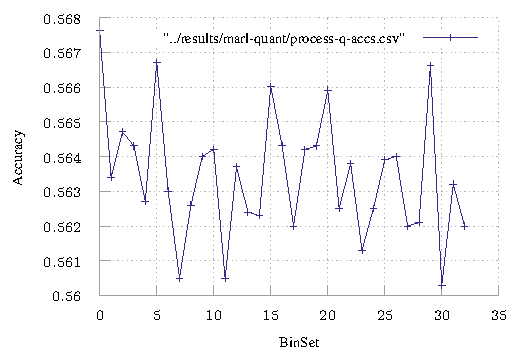
\includegraphics{../plots/build/marl-quant/accuracy-binary}
	\caption{Normalised accuracy of a converted, pre-trained floating-point tile-coded policy after conversion to $32Qn$ fixed-point.}\label{fig:quant-acc}
\end{figure}

\subsubsection{Interaction with stationarity}
Learning time of the system as compared to known changes in normality.

I.e., in the DDoS case: how long does an agent take to respond to the onset of an attack?
A change in attack strategy?
The conclusion of an attack?
There are no citations on \emph{how} DDoS attacks evolve, just that they do, and that this can occur on various timescales.

\subsection{Testbed metrics}
Key (MVP) metrics will be \textbf{bolded}, and expanded with a subsubsection.

\textbf{Traffic throughput (bytes, packets)}, \textbf{packet processing delay}, \textbf{action execution time}, \textbf{learning time}, from-scratch learning accuracy, \textbf{rule installation delay/cost}, host and NIC memory costs, policy installation time, ``accuracy'' in the DDoS case.

\subsubsection{Traffic throughput}
Main research question: does moving RL logic onto the NIC reduce maximum throughput of the NIC, even if calculation is on a different functional unit?
This is relevant in both \si{\byte\per\second} and packets per second.

This is application independent, and would assess whether the RL units (acting independently on the netronome) affect throughput compared with a basic P4 program at different work intensities.
Ideally, this would show no effect on forwarding performance.

\subsubsection{Packet processing delay}
Main research question: does the presence of off-path (but on-chip) RL execution meaningfully increase packet processing delay? How does this compare to a P4 program with an equivalent number of tables? What about to OvS?

\subsubsection{Action execution \& learning time}
Main research question: does moving RL logic from the host to the NIC substantially reduce delays from state measurement, to state receipt, to action computation and installation?
These constitute $t_{1...3}$ discussed above.
Primarily, these need to be looked at using varying policy sizes and distribution across memory regions.

We ideally want these both with and without any acceleration from extra cores on the netronome: the point of this being that we can demonstrate that the system (or a similar NetFPGA system) can scale upwards according to available system resources or demands.

\subsubsection{Rule installation delay/cost.}
Main research question: how long does it take to install rules in the above testbed setups? What is the downtime of so doing?

This is application-dependent: see earlier discussions on rule batching and local extern/hash-table use.

\section{Related Work}

?? A switch/NIC architecture like \textcite{DBLP:conf/hotnets/StephensAS18} would remove the need for hard-coded island-island relationships.

?? Taurus. They can't train online though!~\parencite{DBLP:journals/corr/abs-2002-08987}

?? Do switches~\parencite{DBLP:conf/hotnets/XiongZ19}.
?? Train offline, classical methods targetting all match-action P4 systems (no externs etc).

?? N3IC run NNs on NIC~\parencite{DBLP:journals/corr/abs-2009-02353}, allow packet tagging to occur based on pre-trained BNN~\parencite{DBLP:conf/nips/HubaraCSEB16}.
?? both NFP and NetFPGA.
?? Or as an offload mechanism~\parencite{DBLP:conf/sigcomm/SanvitoSB18,DBLP:journals/corr/abs-1801-05731}.
?? Binary NNs ``more suitable for network hardware''~\parencite{DBLP:journals/corr/MiyashitaLM16}?

?? Can we collect some papers on per-packet ML/RL? Per-packet classification using NNs to build decision trees~\parencite{DBLP:conf/sigcomm/LiangZJS19}

?? RL for congestion control. ~\parencite{DBLP:journals/corr/abs-1910-04054}

?? Arbitrary training enhanced by in-network? General NNs~\parencite{DBLP:conf/micro/LiPAYQPWSEK18}, RL-specfic~\parencite{DBLP:conf/isca/LiLYCSH19}.

\section{Conclusion}
	
%\bibliographystyle{ACM-Reference-Format}
%\bibliography{reference}
\printbibliography
	
\end{document}